%!TEX root = ../report.tex

%
% Architecture
%

\section{Architecture} % (fold)
\label{sec:architecture}

This section present the architecture of the solution that we propose, but before will introduce some technology that is used in the solution.

%!TEX root = ../../report.tex

\subsection{Modern OpenGL} % (fold)
\label{sub:modern_opengl}

Majors changes has been imposed to this library from it's early versions and this section covers the modern version of OpenGL, after version 3.2.

OpenGL is an well known cross-platform Application Programming Interface (API) created by Silicon Graphics Computer Systems with Version 1.0 released in July of 1994 for 3-D Graphics and Imaging. It's a streamlined and hardware-independent interface that can be implemented on manny different types of graphics hardware. It's also independent of the machine's operative and windowing systems.

OpenGL provides a small set of geometric primitives - points, lines, triangles and patches that are specified by their vertices. And from this geometric primitives all geometry is constructed, both in 2D and 3D. 

Shaders ``are special functions that the graphics hardware executes. The best way to think of shaders is as little programs that are specifically compiled for your graphics processing unit''. \cite{shreiner2013opengl}

There are some steps that are performed to render an image. First the model is created from geometric primitives and this data is the input  for the pipline(Vertex Data) in Figure~\ref{fig:OGLPipeline}. 

\begin{figure}[htbp]
	\centering
	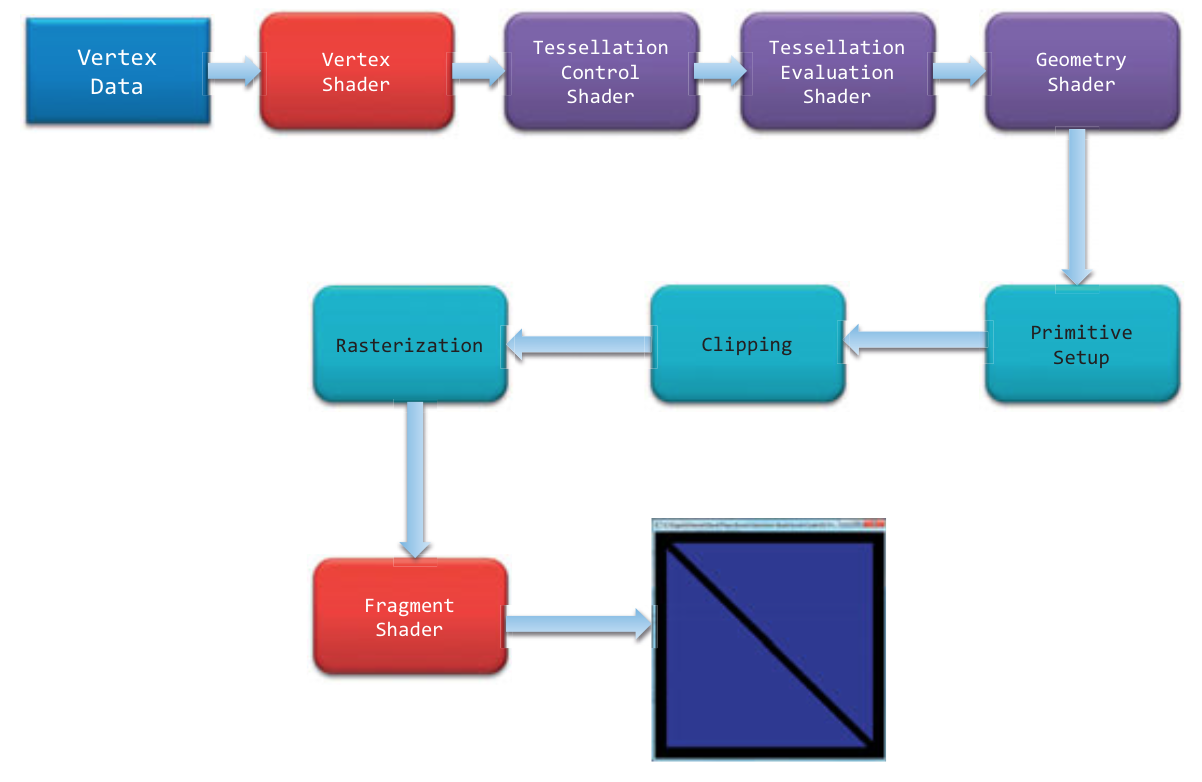
\includegraphics[width=0.95\textwidth]{img/OpenGL/pipeline.png}
	\caption{OpenGL Pipeline \cite{shreiner2013opengl}}
	\label{fig:OGLPipeline}
\end{figure}


The first step of the pipeline is the Vertex Shader that process the data associated with each vertex. 

After this, there are three optional shaders. In this three there are two Tesselation Shaders. With this shaders simple geometries can be tesselated and increase of the number of primitives to improve the models dynamically.

The third optional shader is the Geometric Shader that allows the aditional processing of geometric primitives and also including the creation of new primitives.

Until now all steps work with vertices, and after those steps there are three fixed steps, primitive assembly, clipping and rasterization that assembly the vertices into primitives, clip the geometry cutting the parts that falls of the ``screen'' and the generation of fragments respectively.

A fragments is a ``‘candidate pixel’, in that pixels have a home in the framebuffer, while a fragment still can be rejected and never update its associated pixel location'' \cite{shreiner2013opengl}.
\subsection{Vertex Shaders} % (fold)
\label{sub:vertex_shaders}
Vertex Shaders can be very simple, from a \emph{pass-through shader} that just copies the data to the next step to very complex ones.

In this shaders are used to performed computations to calculate the position of the vertices in screen coordinates, assign vertex's color using lightning computations, etc..

Vertex Shaders have some limitations, they cannot create additional geometry and cannot access data of other vertices. They can just process the data of the current vertex and the number of vertices after this step is the same as before.

% subsection vertex_shaders (end)

\subsection{Tesselation Shaders} % (fold)
\label{sub:tesselation_shaders}
Tesselation Shaders are very different form the previous ones. This shaders address some of limitations presented before.
This shaders work with a geometric primitive called a \emph{patch}.

\subsubsection{Patch} % (fold)
\label{ssub:patch}
	Are lists of vertices that preserves their order during processing. This is because each patch can have an arbitrary number of vertices that have to be specified before drawing oposing to the other primitives that have a specific/pre-assigned/fixed number of vertices.
% subsubsection patch (end)

\subsubsection{Tesselation Control Shader} % (fold)
\label{ssub:tesselation_control_shader}
	This shader generates the tesselation output-patch vertices and specify the tesselation level factors. 

	The output-patch vertices are the list of vertices that results after the input vertices have been processed. 

	The tesselation level factor defines how much the output patch is tesselated. 

	OpenGL supports three tesselation domains: a quadrilateral, a triangle, and a collection of isolines \cite{shreiner2013opengl}. To control the amount of tesselation two sets of values are set, the outer-tesselation values and the inner-tesselation values. This values define how the perimeter or the interior of the domain are subdivided respectivelly.

% subsubsection tesselation_control_shader (end)

\subsubsection{Tesselation Evaluation Shaders} % (fold)
\label{ssub:tesselation_evaluation_shaders}
Tesselation shaders work with the output of the previous phase. Here the vertex positions are calculated from the tessellation computed before. It's is basically responsible for the caclulation of the vertices screen positions from the layout defined.

% subsubsection tesselation_evaluation_shaders (end)

% subsection tesselation_shaders (end)

\subsection{Geometric Shaders} % (fold)
\label{sub:geometric_shaders}

Geometry Shaders are the first shaders that access the complete primitive as a list of vertices and with that it's allowed to do different actions that require this access to information. The amount of output can be variable so both \emph{culling geometry} and \emph{geometry amplification}, respectivelly output less vertices that the input and output more vertices than the input. Also in this shaders the primitives type can be modified, i. e. the input can be \emph{quads} and the output be a \emph{triangle\_strip}.

% subsection geometric_shaders (end)

\subsection{Fragment Shaders} % (fold)
\label{sub:fragment_shaders}
This shaders implement the last phase of the pipeline. Here the fragment's final color is computed and also the depth value.

Fragment Shaders are usefull to implement texture mapping or lights for instance.

% subsection fragment_shaders (end)
% subsection modern_opengl (end)

\subsection{The Proposed Solution} % (fold)
\label{sub:solution}

This work will follow the architecture described in Figure~\ref{fig:architecture}.
There will be a module in Racket that will provide a Racket interface for the rest of the system using \emph{Racket FFI}. 
Is through this interface that users will interact with the system. This will be a layer that will not have an impact on performance.


\begin{wrapfigure}{r}{0.5\textwidth}
	\vspace{-15pt}
    \centering
	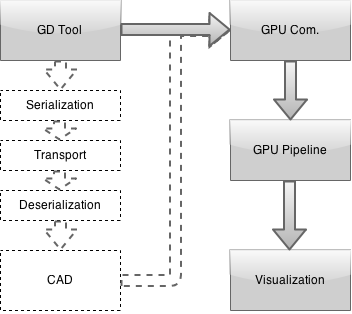
\includegraphics[width=0.5\textwidth]{img/Architecture/GD-Fast-Pipeline.png}
	\caption{High Level Architecture}
	\label{fig:architecture}
	\vspace{-15pt}
\end{wrapfigure}

The second step is the OpenGL layer, that implements the Racket interface and then creates the window and manages user input. The functions provided to
Racket will create here the description of the geometry that will be \emph{amplified} in the next phase. This description is one $GL\_POINT$ that
represent each geometric primitive and is embedded with an array of floats that encode the position, the type of geometry and specific information like
size or number of sides. For example, to create a cylinder, instead of generating all the points that represent a cylinder, that can have $2\times 32$ points, each one with three values so $193$ values in total, we generate a description with only 7 values that encode the primitive type, three values for the position, and three values for the size in each direction.

In the last step are the shaders, where most of the work is done. This receives the small description of the geometry and generates the primitives to be
drawn. To achieve this, it is applied the concept of geometry amplification. As explained in Section~\ref{sub:geometriy_shaders}, this method has
limitations that could make an impact on how the geometry generation is implemented. However OpenGL guarantees support for at least 256 vertices which
is enough to generate the majority of geometric primitives. Since this problem is hardware dependent and GPU hardware is getting more powerful this
should not be a problem in the near future. 
To achieve high performance with this system, will be explored and implemented within this module the concepts of level of detail (LOD) and object
culling. The first is related with the detail which each object is generated in relation with the camera position, generating  objects with high detail
when they are close to the camera and to progressively lose detail when move away from the camera.  At the same time, objects that are partly or
completely covered by other objects are generated in order to decrease the detail or even prevent them from being generated.

This architecture significantly reduces the amount of data that is moved between layers and takes advantage of the power that recent GPUs have. 
In order to validate this architecture, one prototype has been implemented. This prototype currently supports a subset of the geometric primitives: cubes and cylinders.

For instance the following code results in the Figure~\ref{fig:pic1} that is a procedural generated model of a city with ~40k buildings. This example
was generated with the current prototype with the following Racket code:


%\begin{lstlisting}[frame=single,language=Lisp]

\lstset{style=racket}
\begin{lstlisting}
(define (building x y z w l h)
  (let ([h1 (* 0.7 h)]
        [h2 (* 0.4 h)])
    (begin
      (box x y h1 w l h1)
      (cylinder x y (+ (* h1 2) h2) (* 0.7 w) h2))))

(init 1000)

(let ([grid-size 30.0])
  (for* ([xi  (in-range (- grid-size) grid-size 0.3)]
         [yi  (in-range (- grid-size) grid-size 0.3)])
    (building xi yi 0.0 0.1 0.1 (random))))

(start)
\end{lstlisting}
%\begin{absolutelynopagebreak}

%\end{absolutelynopagebreak}

The \emph{init} command makes an initialization of the system and its argument is an estimation of the number of primitives just for optimization
purposes, the \emph{start} command creates the window and starts the visualization. In between the model is created, in this case the code that creates
a squared city model with buildings of random height.

\colocarFiguraMaisRodada

\begin{figure}[htb]
	\centering
	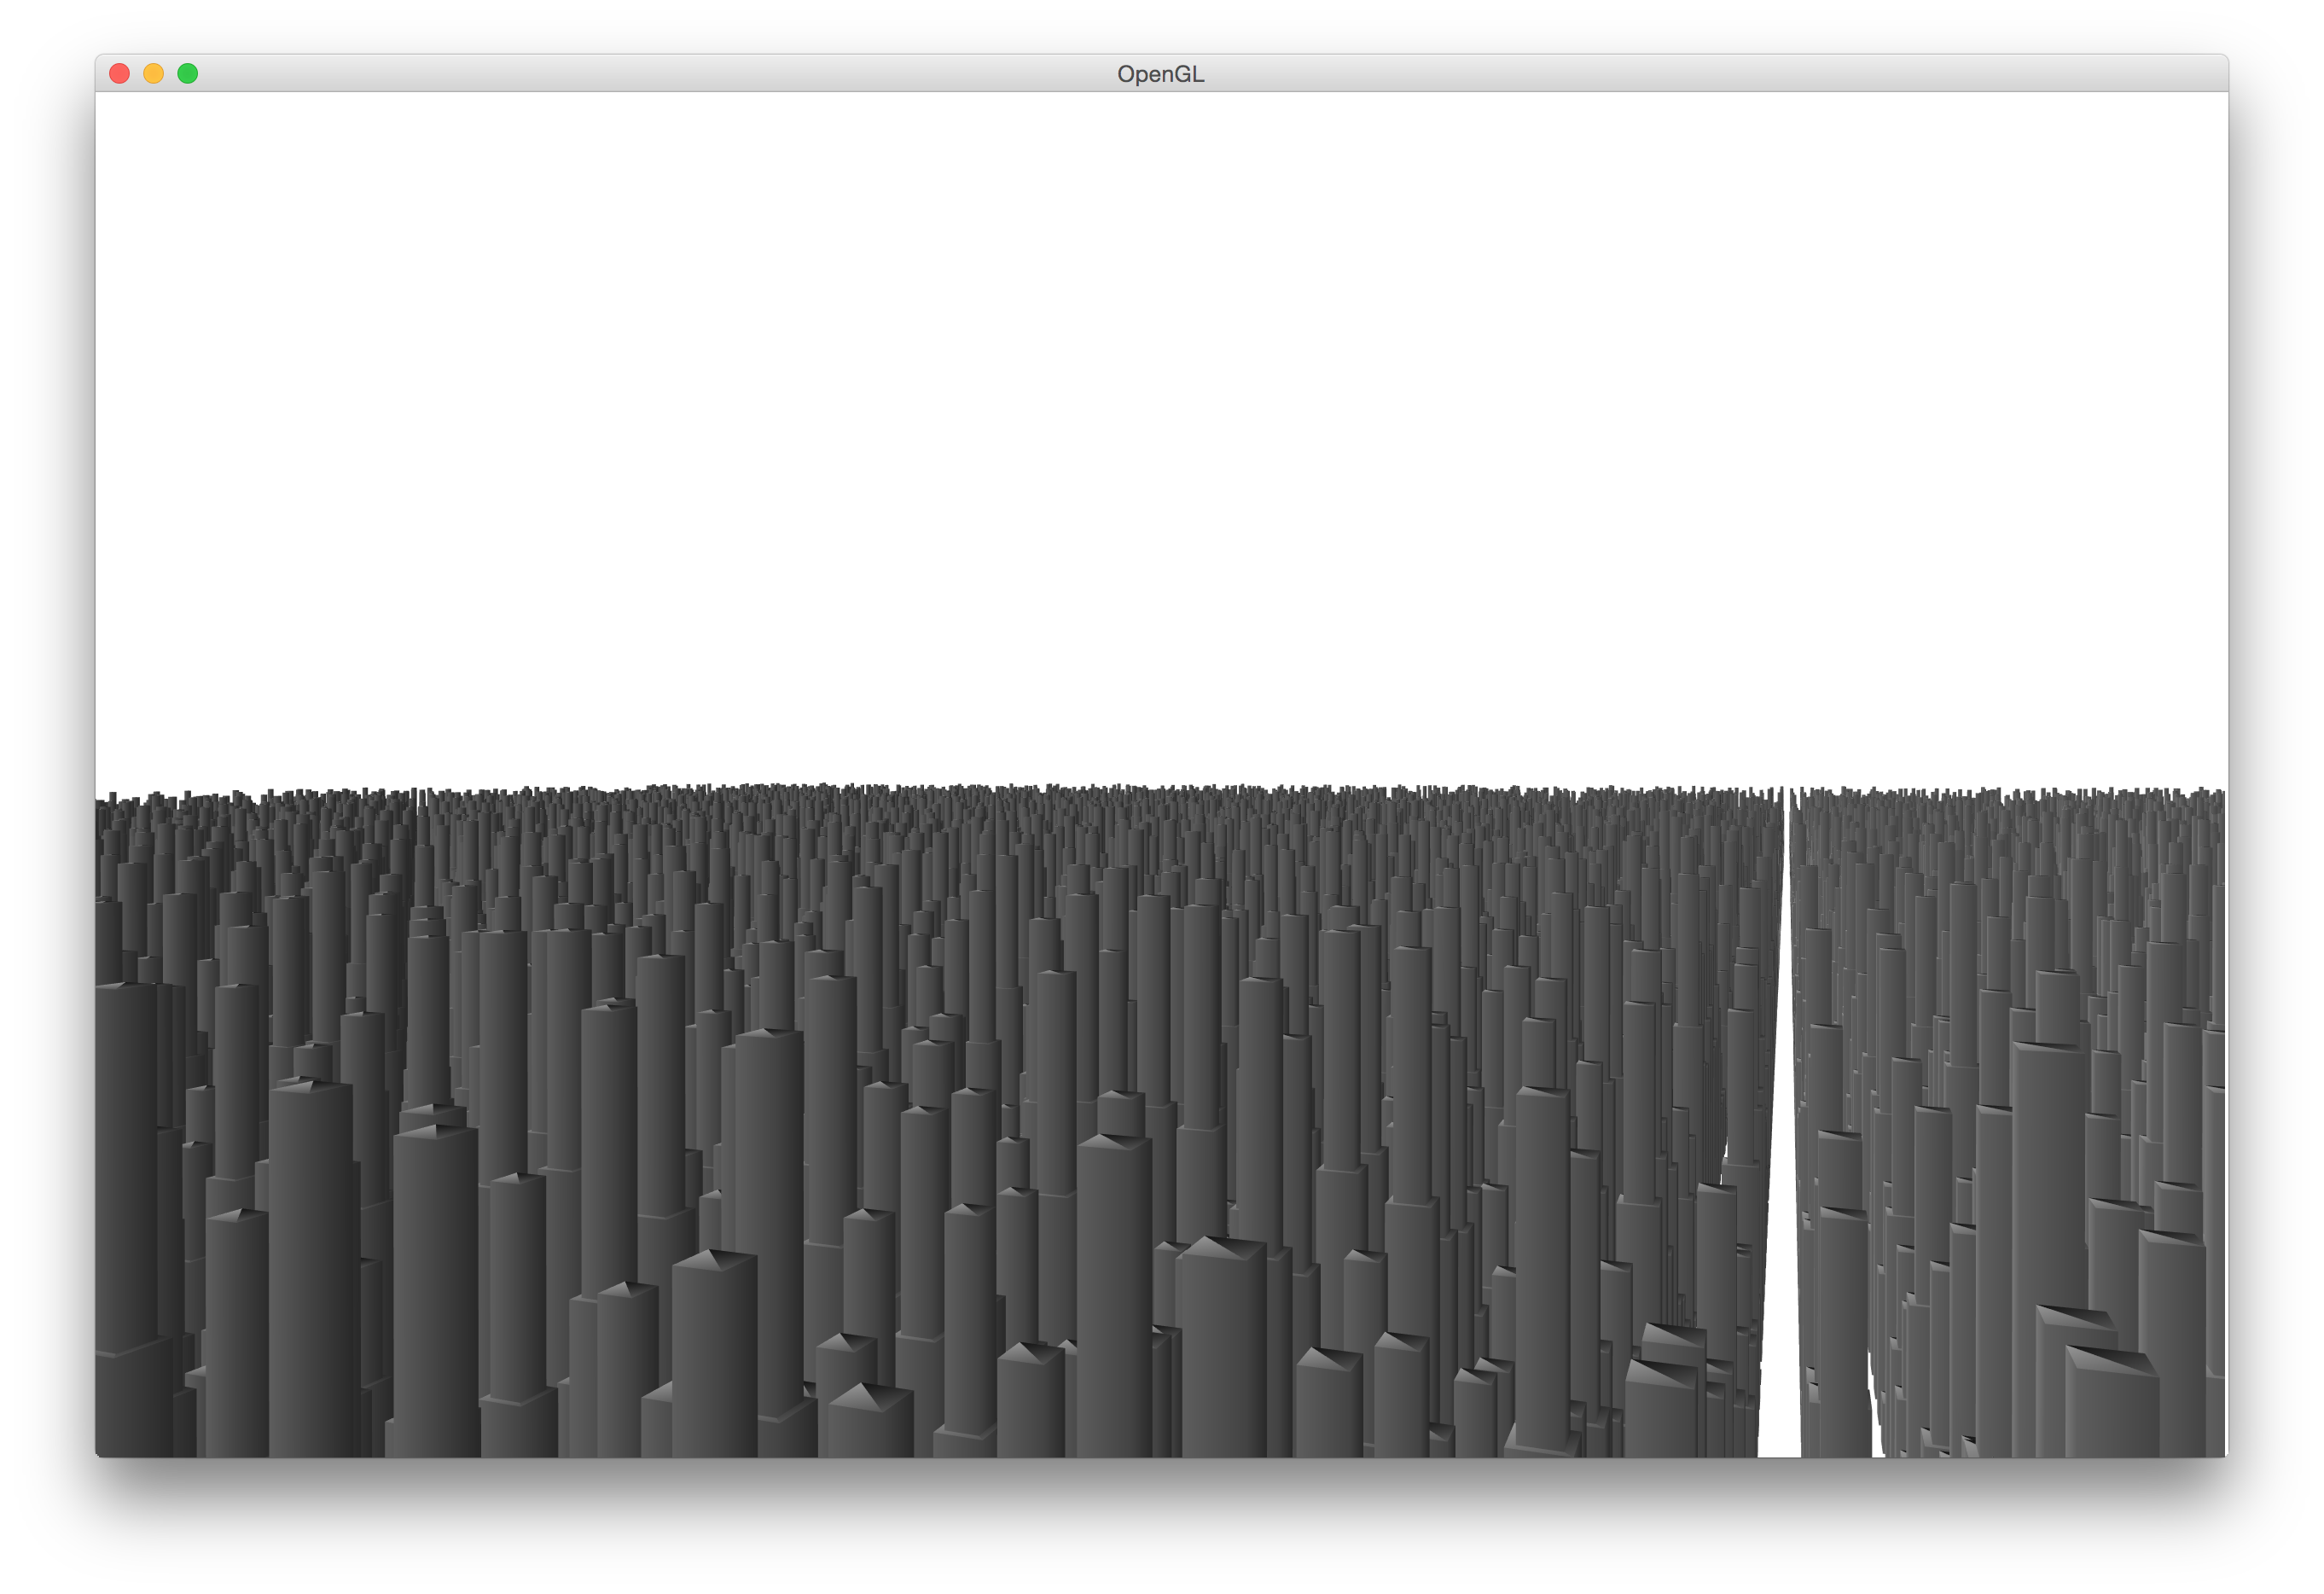
\includegraphics[width=0.95\textwidth]{img/Solution/City5-racket.png}
	\caption{City with ~40k buildings}
	\label{fig:pic1}
\end{figure}



% section architecture (end)
